\documentclass[12pt]{article}
\usepackage[utf8]{inputenc}
\usepackage{listings}
\usepackage{graphicx}
\graphicspath{ {./images/} }
\setlength{\parindent}{0em}
\setlength{\parskip}{1em}

\title{Assignment 8: Expression Lists}
\author{E96C Summer Design Institute}
\date{2020 Session A}

\begin{document}

\maketitle

\section{Introduction}
Welcome to Pointers Assignment 2!

Oh no! All the number keys on my keyboard have stopped working. Also my computer isn't letting me type any mathematical operations (+ - * /).

I need to finish this calculation program I've been working on. Luckily I already implemented the functions to do basic math and defined the words one, two, and three.


\section{Task}
I don't know why, but my boss really wanted me to make a way of expressing a mathematical function as a linked list, and I only have until \_\_\_Due Date\_\_\_ to do it. Basically, I need to have a sequence of nodes, each of which applies a single mathematical operation (such as "add 3" or "divide by 2") and points to whatever the next operation should be. You can tell where the end of the expression is by checking if the "next" value is NULL. By looping through these commands, you can create some pretty crazy expressions.

\begin{center}
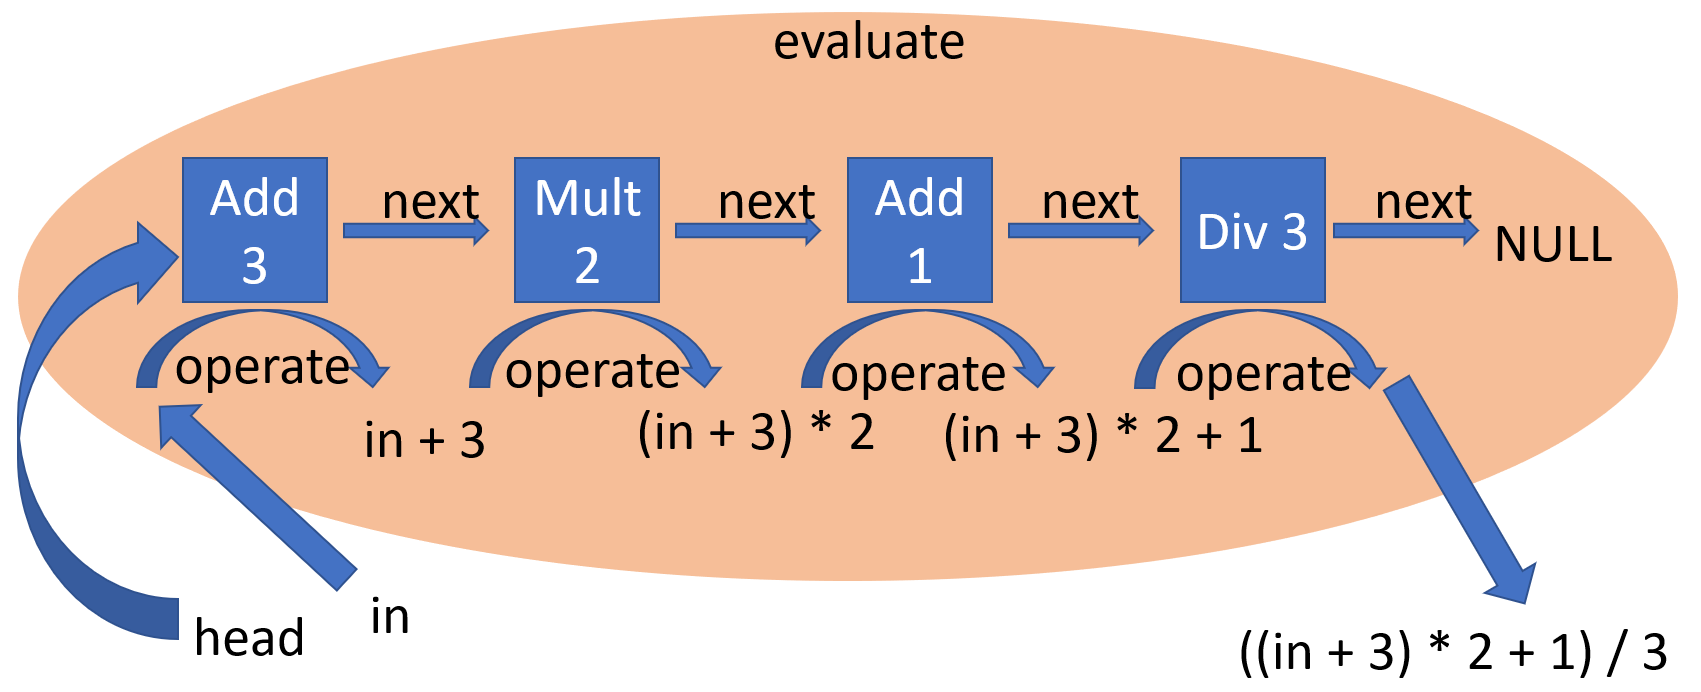
\includegraphics[width=13cm]{images/betterDiagram.png}
\end{center}

\section{Rules}

You are allowed to use -\textgreater  and * as they are relevant to pointers even though they have mathematical operation characters. Do not use them for math.

The expected solution line counts are not requirements, they are suggestions.

You may not type any numbers, but "one", "two", and "three" are already defined for you to use. You can use numbers in your variable names if you want, just not as values.

\section{Notes/Tips}
Using defined values:
Notice how there are several lines which define one, two, and three to their numerical counterparts.
We can use these just like we would those numbers in code.

\begin{lstlisting}[language=C]
#define three 3
int a = three; //a will have value 3
\end{lstlisting}
Make changes to assignment8.c and include your name at the top of the file

We will be testing functions individually to allow for partial credit.

\end{document}
